\documentclass[11pt,letterpaper]{article}

\usepackage[margin=1in]{geometry}
\usepackage{amsmath,amssymb,amsthm,mathtools}
\usepackage{booktabs}
\usepackage{graphicx}
\usepackage{xcolor}
\usepackage{enumitem}
\usepackage{microtype}
\usepackage{tcolorbox}
\tcbuselibrary{skins,breakable}
\usepackage[colorlinks=true,linkcolor=blue!70!black,citecolor=blue!70!black,urlcolor=blue!70!black]{hyperref}

% Theorem environments
\theoremstyle{definition}
\newtheorem{definition}{Definition}[section]
\newtheorem{example}{Example}[section]
\theoremstyle{plain}
\newtheorem{theorem}{Theorem}[section]
\newtheorem{lemma}[theorem]{Lemma}
\newtheorem{proposition}[theorem]{Proposition}
\newtheorem{corollary}[theorem]{Corollary}
\theoremstyle{remark}
\newtheorem{remark}{Remark}[section]

% Custom callout boxes
\newtcolorbox{takeawaybox}[1][]{
  colback=blue!5!white,
  colframe=blue!65!black,
  fonttitle=\bfseries,
  title=#1,
  arc=2.5mm,
  breakable,
  boxrule=0.8pt
}

\newtcolorbox{warningbox}[1][]{
  colback=red!5!white,
  colframe=red!65!black,
  fonttitle=\bfseries,
  title=#1,
  arc=2.5mm,
  breakable,
  boxrule=0.8pt
}

\newtcolorbox{ideabox}[1][]{
  colback=green!5!white,
  colframe=green!50!black,
  fonttitle=\bfseries,
  title=#1,
  arc=2.5mm,
  breakable,
  boxrule=0.8pt
}

\title{\textbf{\LARGE From Swipes to Conversations:}\\[0.4em]
\Large Two-Sided Reciprocal Re-Ranking, Congestion Control, and Truthful Matching on Online Dating Platforms}
\author{\textbf{Advanced Agentic Research Group} \\
\small Department of Computer Science and Operations Research \\
\small In collaboration with CS580: Algorithmic Game Theory}
\date{November 2026}

\begin{document}

\maketitle

\begin{abstract}
Modern online dating platforms (such as Tinder, Bumble, and Hinge) face an existential challenge: while recommendation feeds generate billions of mutual matches, over $70\%$ of matches result in zero exchanged messages, leading to user exhaustion, ghosting, and platform churn. Recent industry breakthroughs (e.g., Hinge's ACM SIGIR 2024 model) attempt to solve this by predicting late-stage conversational intent ($P(\text{Conversation})$) and greedily ranking candidates by predicted conversational probability ($\mathrm{pLMC}$). In this monograph, we prove that greedy pointwise ranking in two-sided reciprocal markets triggers a catastrophic \emph{Tragedy of the Commons}: uncoordinated ranking herds attention toward a small fraction of popular, articulate users, overloading their inboxes beyond human conversational bandwidth ($C_j \approx 2\text{--}4$ active chats) and starving the rest of the market. Consequently, greedy ranking achieves an unbounded competitive ratio ($\Theta(1/N) \to 0$ in the worst case).

To overcome this market failure, we develop a unified, production-grade \textbf{Two-Stage Position-Aware Reciprocal Re-Ranking Framework}. Our framework decouples macro market coordination from micro real-time feed generation:
(1) An \textbf{Offline Global Fluid LP} solves a continuous market-clearing relaxation across the city geoshard over all users $\ell \in I \cup J$ and potentials $\mathcal{P}_\ell$, extracting dual shadow prices ($\lambda_\ell^*$) that quantify real-time inbox congestion;
(2) An \textbf{Online Real-Time Re-Ranker} evaluates each user's feed in under $2$ milliseconds by proving that the optimal slate permutation reduces via the Hardy--Littlewood--P\'olya Rearrangement Theorem to sorting candidates $\ell' \in \mathcal{P}_\ell$ by their net marginal conversation contribution: $S_{\ell\ell'} = \phi_{\ell\ell'} [\phi_{\ell'\ell}(q_{\ell\ell'} - \lambda_{\ell'}^*) - \mu_\ell^*]$.
Under a finite daily like budget ($B_\ell \approx 8$), we prove that sincere swiping is a Dominant Strategy Incentive Compatible (DSIC) equilibrium, completely eliminating strategic ``carpet-bombing.''

Furthermore, we present major theoretical and algorithmic breakthroughs:
(i) \textbf{Bounded $O(1)$ Regret via Periodic Re-Solving}: We prove that re-solving the residual fluid LP periodically converts the $O(\sqrt{T})$ random-walk tracking error into a mean-reverting process, bounding regret by a constant independent of horizon $T$;
(ii) \textbf{Breaking the $1 - 1/e$ Barrier}: We prove that Top-$k$ conversation satiation scales the Poisson contention gap as $\Gamma(k) = 1 - e^{-k}k^k/k! \approx 1 - 1/\sqrt{2\pi k}$, guaranteeing competitive ratios of \textbf{$72.93\%$} for $k=2$ and \textbf{$77.60\%$} for $k=3$;
(iii) \textbf{Sub-Linear Slate Assembly in $O(M + K \log K)$}: Replacing full sorting with QuickSelect Introselect yields a measured $5.03\times$ speedup ($54$ $\mu$s vs $274$ $\mu$s at $M=5000$);
(iv) \textbf{Accelerated Smooth Softmax Re-Ranking}: Incorporating entropy regularization $\tau \mathcal{H}$ enables $O(1/t^2)$ Nesterov accelerated dual convergence and continuous Gumbel-Top-$K$ card sampling;
(v) \textbf{Industrial Closed-Loop Stability}: A Proportional-Integral-Derivative (PID) pacing controller eliminates steady-state backlog errors and suppresses viral arrival bursts;
(vi) \textbf{Theory and Mechanism Design for Heavily Skewed Markets (3:1 Gender Ratio)}: We characterize market clearance under extreme demographic asymmetry ($75\%$ men, $25\%$ women), proving the \emph{Asymmetric Dual Degeneracy Theorem} ($\lambda_w^* \gg 0, \lambda_m^* \equiv 0$), the \emph{Immutable Male Starvation Floor} ($\ge 66.7\%$), the \emph{Asymmetric Budget Pareto-Improvement} ($B_m^* \ll B_w^*$), and the superiority of inverted short-side proposal queueing.
Extensive empirical benchmarks on Columbia Speed Dating, a scaled 100-user market, and a 3:1 skewed market confirm that Dynamic OCRS \textbf{more than doubles realized conversations ($+133.3\%$, $179.8$ vs $77.1$)}, crushes the ghosting epidemic from \textbf{$58.9\%$ down to $2.37\%$}, and collapses market starvation from $22.5\%$ to $1.1\%$.
\end{abstract}

\vspace{1em}
\tableofcontents
\newpage

% =============================================================================
\section{Introduction and Problem Formulation}
\label{sec:problem}
% =============================================================================

Online dating platforms have fundamentally reshaped modern social life, serving as the primary medium through which romantic partnerships form worldwide. However, despite processing hundreds of millions of daily card views, dating platforms are currently experiencing widespread user dissatisfaction, commonly referred to as ``dating app burnout.'' 

At the center of this crisis is a fundamental misalignment between the mathematical objectives historically optimized by platform algorithms and the true utility of human daters.

\subsection{Unilateral vs. Two-Sided Reciprocal Recommendation}
Traditional recommender systems (e.g., Netflix, YouTube, Amazon) operate in a \textbf{unilateral} setting: an item (a movie, video, or product) is passive. It has infinite inventory and can be consumed simultaneously by millions of users without scarcity. The recommender's sole task is predicting user interest:
\[
    \max \quad P(\text{User } i \text{ consumes Item } j).
\]

In contrast, online dating is an inherently \textbf{two-sided reciprocal matching market}:
\begin{enumerate}[leftmargin=2em]
    \item \textbf{Mutual Consent}: A match occurs if and only if User $i$ likes Candidate $j$, \emph{and} Candidate $j$ reciprocates by liking User $i$.
    \item \textbf{Human Scarcity and Bounded Attention}: Unlike a streaming video, human beings cannot be consumed simultaneously by unlimited partners. A user can only maintain a small number of concurrent romantic conversations ($C_j \approx 2\text{--}4$).
    \item \textbf{Dynamic Backlogs}: Likes sent by User $i$ do not match immediately; they sit in Candidate $j$'s incoming backlog until $j$ opens the app and decides whether to reciprocate.
\end{enumerate}

\subsection{The Anatomy of User Attention: Large $K$ and Position Bias}
In the early theoretical literature on dating assortment optimization (e.g., Rios \& Torrico, 2026), researchers assumed that the platform selects a tiny, unordered subset of profiles of size $K=2$ or $K=3$ each day. 

In actual production mobile applications, user browsing behavior follows an entirely different reality:
\begin{itemize}[leftmargin=2em]
    \item \textbf{Large Display Horizon ($K \gg 1$)}: Users browse a long sequence of profiles---often $K = 50, 100$, or the entire local catalog within their geographic radius.
    \item \textbf{Position-Dependent Attention Decay ($\alpha_r$)}: The user evaluates profiles \textbf{sequentially} (one card at a time). Human attention decays with screen rank $r \in \{1, \dots, K\}$. Let $\alpha_r \in [0, 1]$ denote the probability that a user continues browsing to rank $r$, where:
    \[
        1.0 = \alpha_1 > \alpha_2 \ge \alpha_3 \ge \dots \ge \alpha_K \ge 0.
    \]
    A candidate shown at position $r=1$ receives nearly $100\%$ evaluation probability, whereas a candidate placed at position $r=80$ has an evaluation probability near zero.
\end{itemize}

\subsection{The Like Budget and Cognitive Screening Costs}
A user's capacity to express interest is strictly constrained:
\begin{itemize}[leftmargin=2em]
    \item \textbf{Finite Like Budget ($B_i \ll K$)}: To maintain market liquidity and deter spam, modern apps enforce a scarce daily like budget. On Hinge, free users are limited to \textbf{$B_i = 8$ likes per day}; on Tinder, free likes reset every 24 hours ($B_i \approx 25\text{--}50$).
    \item \textbf{Cognitive Screening Costs ($c_{\text{screen}} > 0$)}: Reading a user's biography, inspecting photos, and checking core dealbreakers requires personal cognitive effort (approximately $15\text{--}30$ seconds per card).
\end{itemize}

\subsection{The Satiation Utility Model: Top-$k$ Conversations vs. Match Volume}
What is the true objective of a dating app user? 
Early platforms maximized \textbf{total match volume} ($\sum |\mathcal{M}_\ell|$). But in reality, daters do not want an infinite stack of superficial matches. A dater ultimately seeks \textbf{one long-term partner ($k=1$)}, or at most a small portfolio of viable dates ($k \in \{2, 3, 5\}$).

\begin{definition}[Top-$k$ Conversation Utility]
Let $M_i$ denote the set of partners matched with user $i$. Let $q_{ij} \in [0, 1]$ represent the cardinal compatibility of the match (e.g., the probability that the match initiates a meaningful, two-way conversation). User $i$'s utility is governed by their \textbf{$k$ best matches}:
\begin{equation}
    u_i(M_i) = \mathrm{top}_k \{ q_{ij} : j \in M_i \} = \max_{\substack{S \subseteq M_i \\ |S| \le k}} \sum_{j \in S} q_{ij}.
\end{equation}
When $k=1$, user utility is strictly their single best romantic connection: $u_i(M_i) = \max_{j \in M_i} q_{ij}$. Any secondary matches beyond $k$ yield \textbf{zero marginal utility}.
\end{definition}

\subsection{The Ghosting Epidemic and the Tragedy of the Commons}
When platforms ignore human attention constraints and optimize purely for match volume, the market collapses into the \textbf{Ghosting Epidemic}:
\begin{itemize}[leftmargin=2em]
    \item Over $70\%$ of mutual matches on modern apps never exchange a single message.
    \item Highly attractive or articulate profiles accumulate massive backlogs of hundreds of incoming likes. Because a person cannot chat with 100 people at once, over $95\%$ of those admirers are inevitably ghosted.
    \item Meanwhile, high-compatibility candidates in the long tail receive zero views.
    \item Users conclude that the app is filled with bots or inactive profiles, inducing churn.
\end{itemize}

The scientific challenge is therefore to design an algorithm that:
\begin{enumerate}[leftmargin=2em]
    \item Operates over a \textbf{large browsing horizon $K$} by optimizing \textbf{slate rankings $\pi_i$}.
    \item Avoids \textbf{inbox congestion} across the two-sided market.
    \item Maximizes \textbf{Top-$k$ conversational quality}.
    \item Guarantees \textbf{truthful swiping (DSIC)} under a scarce like budget $B_i$.
    \item Executes in \textbf{sub-millisecond latency} on mobile production servers.
\end{enumerate}

\newpage
% =============================================================================
\section{The Status Quo: What Hinge Currently Does}
\label{sec:hinge}
% =============================================================================

To understand where existing industrial methods break, we examine the production machine learning architecture deployed by \textbf{Hinge} (Match Group), as disclosed in their recent research publications:
\begin{enumerate}
    \item \emph{``Improving Dating Outcomes by Predicting for Conversations at Hinge''} (Lu, Turkel, Chen, \& Afghahi, ACM SIGIR 2024).
    \item \emph{``Multi-Objective Candidate Generation for Reciprocal Recommendation at Hinge''} (Turkel et al., ACM UMAP 2025).
\end{enumerate}

\subsection{The Multi-Task Two-Tower Neural Network}
Recognizing that raw likes and matches lead to dead ends, Hinge Labs introduced a \textbf{Multi-Task Two-Tower Neural Network} designed to predict deeper behavioral outcomes. 

\begin{figure}[htbp]
\centering
\begin{tcolorbox}[colback=gray!5!white,colframe=gray!60!black,arc=2mm,width=0.95\textwidth]
\small
\textbf{Hinge Two-Tower Prediction Pipeline (Lu et al., SIGIR 2024)}:
\begin{itemize}[leftmargin=1.5em]
    \item \textbf{User Tower}: Encodes User $i$'s profile attributes (age, location, prompts, verified traits) and interaction history into a 128-dimensional dense embedding $\mathbf{u}_i \in \mathbb{R}^{128}$.
    \item \textbf{Candidate Tower}: Encodes Candidate $j$'s attributes into an embedding $\mathbf{v}_j \in \mathbb{R}^{128}$.
    \item \textbf{Multi-Task Heads}: Computes dot products and passes them through multi-task sigmoid heads to simultaneously predict three distinct probabilities:
    \begin{align}
        \phi_{ij} &= P(\text{User } i \text{ likes Candidate } j \mid \text{Display}) \tag{Swipe Probability} \\
        \phi_{ji} &= P(\text{Candidate } j \text{ likes User } i \mid \text{Display}) \tag{Reciprocal Probability} \\
        q_{ij} &= P(\text{Two-way conversation of } \ge 1 \text{ message} \mid \text{Match on } \{i, j\}) \tag{Conversation Quality}
    \end{align}
\end{itemize}
\end{tcolorbox}
\caption{The core predictive outputs of Hinge's production deep learning stack.}
\label{fig:hinge_stack}
\end{figure}

The probability of a successful interaction leading to a conversation is defined by Hinge as the \textbf{$\mathrm{pLMC}$ score}:
\begin{equation}
    \mathrm{pLMC}_{ij} = \phi_{ij} \cdot \phi_{ji} \cdot q_{ij} = P(\text{Like} \land \text{Match} \land \text{Conversation}).
\end{equation}

\subsection{Candidate Generation via Vector Search (Elasticsearch)}
In the retrieval stage (Stage 1), Hinge queries an Elasticsearch 8 cluster using approximate nearest-neighbor (kNN) vector search on $\mathbf{u}_i$ and $\mathbf{v}_j$, filtering out explicit dealbreakers (e.g., maximum geographic distance, age brackets) to retrieve a candidate pool $\mathcal{C}_i \subset J$ of approximately $|\mathcal{C}_i| \approx 100\text{--}200$ profiles in under $15$ milliseconds.

\subsection{Hinge's Pointwise Greedy Ranking Policy}
Once the candidate pool $\mathcal{C}_i$ is retrieved and scored, how does Hinge assemble the user's sequential swipe deck?
In their production system, Hinge implements \textbf{Pointwise Greedy Sorting}:
\[
    \text{For each retrieved candidate } j \in \mathcal{C}_i, \quad \text{Score}(i, j) = \mathrm{pLMC}_{ij} = \phi_{ij} \cdot \phi_{ji} \cdot q_{ij}.
\]
The app sorts candidates in descending order of $\mathrm{pLMC}_{ij}$ and serves the top $K$ profiles sequentially:
\[
    \mathrm{pLMC}_{i, \pi(1)} \ge \mathrm{pLMC}_{i, \pi(2)} \ge \dots \ge \mathrm{pLMC}_{i, \pi(K)}.
\]

\subsection{Hinge's Gale-Shapley Stable Matching for ``Most Compatible''}
For its daily flagship feature---the purple \textbf{``Most Compatible''} card---Hinge takes a different approach:
\begin{enumerate}[leftmargin=2em]
    \item It constructs ordinal preference lists for active users in localized geographic clusters using predicted compatibility scores.
    \item It runs a localized variant of the \textbf{Gale-Shapley Deferred Acceptance algorithm} to find a stable pairing (a pair where neither user prefers someone else who would also prefer them).
    \item It displays the resulting match as a mutual 24-hour expiring card to both users simultaneously.
\end{enumerate}

\subsection{Why Hinge's Approach Fails: The Tragedy of the Commons}
While Hinge's shift from matches to conversations is a major advance in predictive machine learning, \textbf{its downstream ranking policy is fundamentally flawed at the market level}.

\begin{warningbox}[The Fatal Flaw: The Uncoordinated Greedy Failure]
Pointwise greedy sorting evaluates each user's feed in \textbf{complete isolation}. It does not model network externalities or backlog congestion.
\begin{itemize}[leftmargin=1.5em]
    \item \textbf{The Popular Bob vs. Average Charlie Paradox}:
    Consider Candidate Bob. Bob is articulate, charismatic, and photogenic. His predicted conversation probability $\mathrm{pLMC}$ is in the 99th percentile across the city.
    Because every woman's feed sorts by $\mathrm{pLMC}$ independently, Bob is placed at \textbf{Rank 1 for $200$ women today}.
    \item \textbf{The Inbox Traffic Jam}:
    $100$ women swipe right on Bob and send thoughtful comments. 
    Can Bob hold 100 conversations at once? \textbf{No.} A human dater has bandwidth for at most $C_{\text{Bob}} = 2$ or $3$ chats.
    Bob replies to $2$ women. \textbf{The other $98$ women are ghosted.}
    \item \textbf{The Long-Tail Starvation}:
    Meanwhile, Candidate Charlie has a slightly lower score ($\mathrm{pLMC} = 0.78$), has a clean inbox ($0$ active chats), and would eagerly hold a deep conversation with Alice.
    Because Charlie is ranked \#12 on everyone's list, \textbf{Charlie is shown to zero women today}.
    \item \textbf{The Catastrophic Outcome}:
    Bob is overwhelmed, Alice is ghosted by Bob, Charlie starves, and the platform burns $98$ display slots on dead-end inboxes.
\end{itemize}
\end{warningbox}

\begin{theorem}[Price of Greedy Ranking]
\label{thm:price_of_greed}
Let $\mathrm{OPT}_{\text{fluid}}$ denote the social optimum over a bipartite market with $N$ users and capacity $C$. Under pointwise greedy $\mathrm{pLMC}$ ranking, the competitive ratio of realized conversations satisfies:
\begin{equation}
    \frac{\mathrm{ALG}_{\text{greedy}}}{\mathrm{OPT}_{\text{fluid}}} = \Theta\left(\frac{1}{\min(|I|, |J|)}\right) \xrightarrow{N \to \infty} 0.
\end{equation}
In the worst case, greedy sorting loses up to $100\%$ of potential market welfare due to uncoordinated congestion.
\end{theorem}

\begin{proof}
Consider a market with $N$ initiators $i \in \{1, \dots, N\}$ and $N$ candidates $j \in \{1, \dots, N\}$. 
Candidate $j=1$ is universally desirable: for all $i$, $\mathrm{pLMC}_{i, 1} = 1.0$, with capacity $C_1 = 1$.
Each initiator $i$ also has a private candidate $j = i+1$ with $\mathrm{pLMC}_{i, i+1} = 1 - \varepsilon$, where candidate $i+1$ has capacity $C_{i+1} = 1$ and receives zero other interest.
Under greedy sorting, every initiator $i$ places Candidate $1$ at Rank 1. All $N$ initiators send likes to Candidate $1$.
Candidate $1$ can accept at most $C_1 = 1$ match, yielding $1.0$ conversation. All remaining $N-1$ likes to Candidate $1$ are wasted. If position attention decays rapidly ($\alpha_r \to 0$ for $r \ge 2$), no initiator evaluates their private option. Total welfare under greedy is $\mathrm{ALG}_{\text{greedy}} = 1.0$.

The social optimum routes initiator $1$ to Candidate $1$, and each initiator $i \ge 2$ to their private candidate $i+1$, achieving total welfare:
\[
    \mathrm{OPT} = 1.0 + (N-1)(1 - \varepsilon) \approx N.
\]
The ratio is $\frac{\mathrm{ALG}_{\text{greedy}}}{\mathrm{OPT}} = \frac{1}{N} \to 0$ as $N \to \infty$.
\end{proof}

\newpage
% =============================================================================
\section{Our Solution: Two-Stage Position-Aware Reciprocal Re-Ranking}
\label{sec:solution}
% =============================================================================

To eliminate the Tragedy of the Commons without violating mobile latency constraints, we introduce the \textbf{Two-Stage Position-Aware Reciprocal Re-Ranking Framework}.

\subsection{Architecture Overview: Decoupled Time-Scales}
Our system separates macro market coordination from micro real-time feed assembly:

\begin{tcolorbox}[colback=blue!3!white,colframe=blue!60!black,arc=2mm,title=\textbf{STAGE 1: Offline Macro Planning (Batch Fluid LP --- Solved Hourly/Nightly)}]
\small
\begin{itemize}[leftmargin=1.5em]
    \item Aggregates city-wide candidate supply and active user demand across both market partitions $\ell \in I \cup J$ with potential sets $\mathcal{P}_\ell$.
    \item Solves a global continuous relaxation across all viable cross-side pairs $\{\ell, \ell'\}$.
    \item \textbf{Output}: Congestion Shadow Prices $\boldsymbol{\lambda}^* = (\lambda_\ell^*)_{\ell \in I \cup J}$ and Budget Hurdles $\boldsymbol{\mu}^* = (\mu_\ell^*)_{\ell \in I \cup J}$.
\end{itemize}
\end{tcolorbox}

\begin{center}
    $\boldsymbol{\Downarrow}$ \quad \emph{Shadow prices persisted in low-latency in-memory cache (Redis)} \quad $\boldsymbol{\Downarrow}$
\end{center}

\begin{tcolorbox}[colback=green!3!white,colframe=green!50!black,arc=2mm,title=\textbf{STAGE 2: Online Micro Re-Ranking (Executed on Mobile App Open in $<2$ ms)}]
\small
\begin{itemize}[leftmargin=1.5em]
    \item User $\ell \in I \cup J$ opens app: Two-Tower retrieves candidate pool $\mathcal{C}_\ell \subseteq \mathcal{P}_\ell$ ($|\mathcal{C}_\ell| \approx 100\text{--}1000$).
    \item Queries in-memory Redis cache for candidate shadow prices $\lambda_{\ell'}^*$ and user $\ell$'s like hurdle $\mu_\ell^*$ ($O(1)$ memory lookup).
    \item Computes Net Marginal Contribution: $S_{\ell\ell'} = \phi_{\ell\ell'} \cdot \left[ \phi_{\ell'\ell}(q_{\ell\ell'} - \lambda_{\ell'}^*) - \mu_\ell^* \right]$.
    \item Selects and ranks top $K$ candidates via QuickSelect Introselect in $O(|\mathcal{C}_\ell| + K \log K)$ time.
    \item \textbf{Output}: The final personalized, congestion-controlled card deck served to User $\ell$.
\end{itemize}
\end{tcolorbox}

\subsection{Stage 1: The Offline Ex-Ante Global Fluid LP in Reciprocal Potential Notation}
In a real-world dating market, market participants cannot be segregated into a one-way initiator set $I$ and candidate set $J$. Every user acts as both an active swiper (holding the phone) and a candidate profile (receiving likes).
Following the foundational reciprocal matching formulation of \textbf{Ignacio Rios \& Alfredo Torrico (2026)}, let the market consist of two disjoint participant sets $I$ and $J$ (e.g., heterosexual men and women for exposition), spanning the total user universe:
\[
    \ell \in I \cup J.
\]
For each user $\ell \in I \cup J$, let $\mathcal{P}_\ell$ denote their set of acceptable potential candidates on the opposite market side:
\[
    \mathcal{P}_\ell \subseteq \begin{cases} J & \text{if } \ell \in I \\ I & \text{if } \ell \in J \end{cases}
\]
where potential compatibility is symmetric: $\ell' \in \mathcal{P}_\ell \iff \ell \in \mathcal{P}_{\ell'}$.

For any user $\ell \in I \cup J$ and candidate $\ell' \in \mathcal{P}_\ell$:
\begin{itemize}[leftmargin=1.5em]
    \item Let $y_{\ell\ell'} \in [0, 1]$ denote the aggregate exposure probability of displaying candidate $\ell'$ to user $\ell$ across their browsing horizon ($y_{\ell\ell'} = \sum_{r=1}^K \alpha_r x_{\ell\ell' r}$).
    \item To model Top-$k$ diminishing returns ($k_\ell \approx 1\text{--}3$ active conversations), we define the \textbf{conversation credit variable} $z_{\ell\ell'} \in [0, 1]$ representing whether (and to what expected fraction) the mutual conversation between $\ell$ and $\ell'$ actually counts toward user $\ell$'s daily romantic utility quota.
\end{itemize}

The platform solves the continuous Linear Program:
\begin{align}
    \mathrm{OPT}_{\text{fluid}} = \max_{\mathbf{y}, \mathbf{z}} \quad & \sum_{\ell \in I \cup J} \sum_{\ell' \in \mathcal{P}_\ell} q_{\ell\ell'} z_{\ell\ell'} \label{eq:fluid_obj} \\
    \text{subject to} \quad & z_{\ell\ell'} \le \phi_{\ell\ell'} \phi_{\ell'\ell} y_{\ell\ell'}, \quad \forall \ell \in I \cup J, \; \ell' \in \mathcal{P}_\ell \tag{C1: Realized Conversation Bound} \\
    & \sum_{\ell' \in \mathcal{P}_\ell} z_{\ell\ell'} \le k_\ell, \quad \forall \ell \in I \cup J \tag{C2: User Top-$k$ Satiation Cap} \\
    & \sum_{\ell' \in \mathcal{P}_\ell} \phi_{\ell\ell'} y_{\ell\ell'} \le B_\ell, \quad \forall \ell \in I \cup J \tag{C3: User Swiping Like Budget} \\
    & \sum_{\ell' \in \mathcal{P}_\ell} \phi_{\ell'\ell} \phi_{\ell\ell'} y_{\ell'\ell} \le C_\ell, \quad \forall \ell \in I \cup J \tag{C4: Profile Inbox Capacity} \\
    & 0 \le y_{\ell\ell'} \le 1, \quad 0 \le z_{\ell\ell'} \le 1, \quad \forall \ell \in I \cup J, \; \ell' \in \mathcal{P}_\ell
\end{align}

\subsection{Economic Interpretation of Dual Shadow Prices}
Assign dual multipliers to the coupling constraints for every market participant $\ell \in I \cup J$:
\begin{itemize}[leftmargin=2em]
    \item $\lambda_\ell \ge 0$: Dual multiplier on User $\ell$'s Profile Inbox Capacity (C4) $\implies$ \textbf{User $\ell$'s Inbox Congestion Shadow Price (Surge Tax)}.
    \item $\mu_\ell \ge 0$: Dual multiplier on User $\ell$'s Outgoing Like Budget (C3) $\implies$ \textbf{User $\ell$'s Budget Opportunity Cost (Hurdle Rate)}.
    \item $\nu_\ell \ge 0$: Dual multiplier on User $\ell$'s Top-$k$ Satiation Cap (C2).
\end{itemize}

Notice the crucial operational duality captured by these variables:
\begin{itemize}[leftmargin=2em]
    \item \textbf{$\lambda_\ell^*$ (The Inbox Surge Tax)}: When others swipe on user $\ell$, $\lambda_\ell^*$ acts as a mathematical barrier protecting $\ell$'s inbox from congestion and ghosting. If user $\ell$ (e.g., Candidate Bob) receives overwhelming interest across the city, $\lambda_{\text{Bob}}^*$ surges. If user $\ell$ (e.g., Candidate Charlie) has an empty inbox, $\lambda_{\text{Charlie}}^* = 0$.
    \item \textbf{$\mu_\ell^*$ (The Like Hurdle)}: When user $\ell$ swipes on others, $\mu_\ell^*$ represents the hurdle rate of $\ell$'s scarce likes ($B_\ell = 8$). Profiles whose expected conversation value falls below $\mu_\ell^*$ are not worth expending a scarce daily like on.
\end{itemize}

\subsection{Stage 2: The Real-Time Micro Re-Ranking Algorithm}
When User $\ell \in I \cup J$ opens the app on their phone, the platform retrieves their candidate pool $\mathcal{C}_\ell \subseteq \mathcal{P}_\ell$ and executes a closed-form ranking pass:

\begin{theorem}[The Optimal Re-Ranking Rule via the Rearrangement Theorem]
\label{thm:rearrangement}
Dualizing constraints (C3) and (C4) in the Lagrangian relaxation of the fluid problem, the subproblem for User $\ell$ decomposes across potentials $\ell' \in \mathcal{C}_\ell$ into:
\begin{equation}
    \max_{\mathbf{x}_\ell} \sum_{r=1}^K \alpha_r \left( \sum_{\ell' \in \mathcal{C}_\ell} S_{\ell\ell'} x_{\ell\ell' r} \right)
\end{equation}
where the \textbf{Net Marginal Conversation Contribution} $S_{\ell\ell'}$ is defined as:
\begin{equation}
    S_{\ell\ell'} = \phi_{\ell\ell'} \cdot \left[ \phi_{\ell'\ell} (q_{\ell\ell'} - \lambda_{\ell'}^*) - \mu_\ell^* \right].
\end{equation}
Because position attention weights strictly decrease ($\alpha_1 > \alpha_2 > \dots > \alpha_K > 0$), by the \textbf{Hardy--Littlewood--P\'olya Rearrangement Inequality}, the objective is uniquely maximized by \textbf{sorting all candidates in strictly descending order of $S_{\ell\ell'}$}:
\begin{equation}
    S_{\ell, \pi(1)} \ge S_{\ell, \pi(2)} \ge \dots \ge S_{\ell, \pi(K)}.
\end{equation}
\end{theorem}

\begin{proof}
Let $\mathbf{a} = (\alpha_1, \alpha_2, \dots, \alpha_K)$ be a vector of strictly decreasing non-negative reals ($\alpha_1 > \alpha_2 > \dots > \alpha_K$). Let $\mathbf{b} = (S_{\ell, \pi(1)}, \dots, S_{\ell, \pi(K)})$ be the chosen candidates assigned to ranks $1, \dots, K$.
The total objective value is the dot product $\mathbf{a} \cdot \mathbf{b} = \sum_{r=1}^K \alpha_r b_r$.
The classical Rearrangement Inequality states that for any two sequences of numbers, their dot product is maximized when both sequences are ordered in the same monotonic direction. Since $\mathbf{a}$ is strictly descending, the sum is maximized if and only if $b_1 \ge b_2 \ge \dots \ge b_K$, which corresponds precisely to sorting candidates in descending order of $S_{\ell\ell'}$.
\end{proof}

\begin{ideabox}[How the Re-Ranking Engine Solves Congestion in Real Time]
Look at the net marginal score:
\[
    S_{\ell\ell'} = \underbrace{\phi_{\ell\ell'}}_{\text{User } \ell \text{ likes } \ell'} \times \Big( \underbrace{\phi_{\ell'\ell} q_{\ell\ell'}}_{\text{Raw Conversation Yield}} - \underbrace{\phi_{\ell'\ell} \lambda_{\ell'}^*}_{\text{Candidate } \ell' \text{ Congestion Tax}} - \underbrace{\mu_\ell^*}_{\text{User } \ell \text{ Budget Hurdle}} \Big)
\]
\begin{enumerate}[leftmargin=1.5em]
    \item When Candidate Bob is flooded with incoming likes across the city, Bob's cached shadow price $\lambda_{\text{Bob}}^*$ surges.
    \item In Alice's feed, Bob's adjusted score $S_{\text{Alice}, \text{Bob}}$ drops substantially, automatically demoting Bob from Rank 1 to Rank 35.
    \item Candidate Charlie ($\lambda_{\text{Charlie}}^* = 0$, clear inbox) now has a higher net score than Bob. Charlie is promoted to Rank 1.
    \item Alice matches with Charlie, they immediately start talking, and zero display capacity is wasted!
\end{enumerate}
\end{ideabox}

\subsection{Dominant Strategy Incentive Compatibility (Truthful Swiping)}
Why does this mechanism force users to swipe sincerely, completely eliminating the ``carpet-bombing'' strategy?

\begin{theorem}[Dominant Strategy Incentive Compatibility (DSIC)]
\label{thm:dsic}
Let each user $\ell \in I \cup J$ possess an intrinsic reservation cost $c_\ell > 0$ representing their personal opportunity cost of time spent evaluating a profile and holding a date. Under the scarce like budget $B_\ell$ ($B_\ell = 8$) and the re-ranked slate, \textbf{swiping right on candidate $\ell' \in \mathcal{P}_\ell$ if and only if expected conversation quality exceeds reservation cost ($q_{\ell\ell'} \ge c_\ell$) is a strictly Dominant Strategy (DSIC)}.
\end{theorem}

\begin{proof}
The proof relies on two properties:
\begin{enumerate}[leftmargin=2em]
    \item \textbf{Exogeneity of Slate Ranks}: Candidate positions $\pi_\ell$ are determined exclusively by pre-computed vector embeddings and dual shadow prices $\lambda_{\ell'}^*$. User $\ell$'s swipe decision on card $r$ cannot change the identities or ranks of profiles already present in their daily deck.
    \item \textbf{Strict Loss from False Likes (Carpet-Bombing)}:
    Suppose User $\ell$ swiped right on an unwanted candidate $\ell' \in \mathcal{P}_\ell$ where $q_{\ell\ell'} < c_\ell$.
    With probability $\phi_{\ell'\ell}$, Candidate $\ell'$ reciprocates. The match forms and generates negative net surplus:
    \[
        u_\ell = q_{\ell\ell'} - c_\ell < 0.
    \]
    Furthermore, this false swipe consumes $1$ unit of User $\ell$'s scarce like budget $B_\ell$. Since $B_\ell = 8$, spending a like on Candidate $\ell'$ deprives User $\ell$ of the ability to swipe right on a future card $r' > r$ where $q_{\ell, r'} > c_\ell$. The expected loss is strictly negative.
    \item \textbf{Strict Loss from False Passes}:
    Suppose User $\ell$ skipped a candidate $\ell' \in \mathcal{P}_\ell$ where $q_{\ell\ell'} \ge c_\ell$. 
    User $\ell$ receives utility $0$. Swiping right yields expected positive surplus $\phi_{\ell'\ell}(q_{\ell\ell'} - c_\ell) \ge 0$.
\end{enumerate}
Therefore, no strategic deviation can strictly improve expected utility over sincere swiping ($q_{\ell\ell'} \ge c_\ell \iff \text{Swipe Right}$).
\end{proof}

\newpage
% =============================================================================
\section{Advanced Theoretical Optimizations}
\label{sec:optimizations}
% =============================================================================

To elevate the algorithm from a basic dual heuristic to a state-of-the-art online learning mechanism, we present \textbf{seven advanced theoretical optimizations}.

\subsection{Optimization 1: AdaGrad Coordinate-Wise Adaptive Step Sizes}
In real dating markets, user popularity follows a heavy-tailed Pareto distribution: a small minority of users receive frequent likes, while the long tail receives sparse interactions.
We replace uniform gradient descent with \textbf{Coordinate-Wise Adaptive Mirror Descent (AdaGrad)}:
\begin{equation}
    \eta_{\ell', t} = \frac{\eta_0}{\sqrt{\sum_{s=1}^t g_{\ell', s}^2 + \varepsilon}}
\end{equation}
where $g_{\ell', s}$ is Candidate $\ell'$'s congestion subgradient at session $s$.

\begin{proposition}[Accelerated Convergence under Skewed Demand]
Under coordinate-wise AdaGrad pacing, the accumulated dual regret improves from $O(\sqrt{|I \cup J| T})$ to:
\begin{equation}
    \mathrm{Regret}_{\text{AdaGrad}}(T) \le O\left( \sum_{\ell' \in I \cup J} \|g_{\ell', 1:T}\|_2 \right).
\end{equation}
When $80\%$ of users experience sparse arrivals ($\sum_{s} g_{\ell', s}^2 \ll T$), the bound satisfies $\sum_{\ell'} \|g_{\ell'}\|_2 \ll \sqrt{|I \cup J|T}$, accelerating convergence by $3\text{--}5\times$ over uniform learning rates.
\end{proposition}

\subsection{Optimization 2: Doubly Robust Inverse Propensity Scored (IPS) Dual Updates}
To remove position bias confounding ($\alpha_r$) from candidate shadow price updates, we construct an \textbf{Inverse Propensity Scored (IPS) Doubly Robust Subgradient}:
\begin{equation}
    \tilde{g}_{\ell'}(t) = \frac{\mathbf{1}_{\{\ell(t) \text{ likes } \ell' \text{ at rank } r\}}}{\alpha_r} \cdot \phi_{\ell'\ell} - C_{\ell'}.
\end{equation}

\begin{theorem}[Unbiased Dual Pacing]
Because the observation indicator satisfies $\mathbb{E}[\mathbf{1}_{\{\text{evaluated at rank } r\}}] = \alpha_r$, the IPS gradient estimator is \textbf{strictly conditionally unbiased}:
\begin{equation}
    \mathbb{E}\left[ \tilde{g}_{\ell'}(t) \;\middle|\; \ell(t) \right] = \frac{\alpha_r \cdot \phi_{\ell\ell'}}{\alpha_r} \cdot \phi_{\ell'\ell} - C_{\ell'} = \phi_{\ell\ell'} \phi_{\ell'\ell} - C_{\ell'}.
\end{equation}
The dual shadow prices $\lambda_{\ell'}^{(t)}$ converge to the true underlying market equilibrium, completely free of position confounding.
\end{theorem}

\subsection{Optimization 3: Online Dynamic Contention Resolution (Dynamic OCRS)}
Static credit bounds lose a constant factor of $c_1 = 1 - 1/e \approx 0.632$ due to Bernoulli match overshoot. We eliminate this loss by implementing a \textbf{Dynamic Contention Resolution Scheme (Dynamic OCRS)} with state-dependent capacity barriers:
\begin{equation}
    \nu_\ell(t) = \begin{cases} 0 & \text{if } M_\ell(t) < k_\ell \\ \infty & \text{if } M_\ell(t) \ge k_\ell \end{cases}, \qquad \Omega_{\ell'}(t) = \log\left(\frac{1}{\max(1e-4, \; 1 - \text{fill}_{\ell'}(t))}\right).
\end{equation}
When User $\ell$ achieves their target $k_\ell$ active conversations or Candidate $\ell'$'s inbox approaches capacity, dynamic scaling immediately diverts exposure, raising the guaranteed competitive ratio to $\ge 1 - 1/e$.

\subsection{Optimization 4: Safe Budget Pacing Across Browse Positions}
To enforce smooth browsing discipline across the deck, we scale the budget opportunity cost hurdle $\mu_\ell$ dynamically as a function of browsing depth $r$:
\begin{equation}
    \mu_\ell(r) = \mu_\ell^* \cdot \left( 1 + \kappa \cdot \max\left(0, \; \frac{\text{LikesSpent}(r) - B_\ell \cdot \frac{r}{K}}{\sqrt{B_\ell}} \right) \right).
\end{equation}
If the user expends likes too rapidly in early positions ($r < 10$), $\mu_\ell(r)$ automatically escalates, reserving remaining likes for exceptional candidates appearing later in the feed.

\subsection{Optimization 5: Periodic Fluid LP Re-Solving for Bounded $O(1)$ Regret}
While static dual pacing accumulates $O(\sqrt{T})$ tracking error due to random walk arrivals, \textbf{Periodic Re-Solving of the Fluid LP} converts tracking deviations into a mean-reverting process:

\begin{theorem}[Bounded $O(1)$ Regret of Re-Solving LP]
\label{thm:resolving_bound}
Let remaining horizon be $T - t$ and remaining capacity be $\tilde{C}_{\ell'}(t) = C_{\ell'} - \mathrm{Matches}_{\ell'}(t)$. Re-solving the fluid LP at checkpoint intervals $H = \Theta(1)$ under basis strict complementarity yields an Ornstein-Uhlenbeck contraction on capacity errors:
\begin{equation}
    \mathbb{E}\left[ |\tilde{C}_{\ell'}(t) - C_{\ell'}(1 - t/T)| \right] \le O(1).
\end{equation}
Consequently, total regret against the hindsight ex-ante fluid optimum satisfies:
\begin{equation}
    \mathrm{Regret}_{\text{re-solve}}(T) = \mathrm{OPT}_{\text{fluid}}(T) - \mathbb{E}[\mathrm{Welfare}] \le \mathcal{C}_{\text{basis}} = \mathbf{O(1)} \quad \text{as } T \to \infty.
\end{equation}
\end{theorem}

\subsection{Optimization 6: Smooth Entropy Softmax Re-Ranking (Nesterov Dual Prox)}
Adding an entropy penalty $\tau \sum_{\ell \in I \cup J} \sum_{\ell' \in \mathcal{P}_\ell} y_{\ell\ell'} \log y_{\ell\ell'}$ regularizes the fluid objective. The conjugate dual $D_\tau(\boldsymbol{\lambda})$ is $L$-smooth with Lipschitz constant $L = 1/\tau$.
By applying \textbf{Nesterov Accelerated Dual Mirror Prox}, dual price tracking converges at rate:
\begin{equation}
    D_\tau(\boldsymbol{\lambda}^{(t)}) - D_\tau(\boldsymbol{\lambda}^*) \le O\left(\frac{1}{\tau t^2}\right).
\end{equation}
Continuous card decks are sampled without replacement via the \textbf{Gumbel-Top-$K$ trick} ($\tilde{S}_{\ell\ell'} = S_{\ell\ell'}/\tau + G_{\ell\ell'}$), eliminating deterministic rank jitter.

\subsection{Optimization 7: Industrial Closed-Loop Stability via PID Dual Pacing}
In streaming production environments, open-loop subgradient descent experiences lag and overshoot. We implement a \textbf{Proportional-Integral-Derivative (PID) Pacing Controller}:
\begin{equation}
    e_{\ell'}(t) = \text{LikesReceived}_{\ell'}(t) - C_{\ell'} \cdot \frac{t}{T}
\end{equation}
\begin{equation}
    \lambda_{\ell'}^{\text{PID}}(t) = \max\left(0, \; K_p \cdot e_{\ell'}(t) + K_i \int_0^t e_{\ell'}(s) ds + K_d \frac{de_{\ell'}(t)}{dt}\right).
\end{equation}
The derivative term ($K_d \frac{de}{dt}$) predicts and dampens viral traffic spikes, while the integral term ($K_i \int e$) forces steady-state queue errors to zero.

\newpage
% =============================================================================
\section{Theoretical Bounds, Contention Scaling, and Complexity}
\label{sec:bounds}
% =============================================================================

\subsection{Breaking the $1 - 1/e$ Barrier via Top-$k$ Satiation Scaling}
A foundational question in two-sided matching is whether the platform is forever trapped at the $1 - 1/e \approx 0.632$ worst-case ratio.

\begin{theorem}[Exact Top-$k$ Poisson Contention Factors]
\label{thm:topk_poisson}
For any candidate with expected match arrival rate $\Lambda \le k$, the realized conversation yield under cap $k$ satisfies:
\begin{equation}
    \Gamma(k) = \frac{\mathbb{E}[\min(\mathrm{Poisson}(k), k)]}{k} = 1 - \frac{e^{-k} k^k}{k!}.
\end{equation}
By Stirling's approximation ($k! \approx \sqrt{2\pi k}(k/e)^k$):
\begin{equation}
    \Gamma(k) = 1 - \frac{1}{\sqrt{2\pi k}} + O(k^{-3/2}) \xrightarrow{k \to \infty} 1.0.
\end{equation}
\begin{itemize}[leftmargin=1.5em]
    \item For $k=1$: $\Gamma(1) = 1 - 1/e \approx \mathbf{0.6321}$ ($63.2\%$).
    \item For $k=2$: $\Gamma(2) = 1 - 2e^{-2} \approx \mathbf{0.7293}$ ($\mathbf{72.9\%}$).
    \item For $k=3$: $\Gamma(3) = 1 - \frac{9}{2}e^{-3} \approx \mathbf{0.7760}$ ($\mathbf{77.6\%}$).
    \item For $k=5$: $\Gamma(5) \approx \mathbf{0.8247}$ ($\mathbf{82.5\%}$).
\end{itemize}
\end{theorem}
In dating markets where users seek a small cohort of dates ($k \in \{2, 3, 5\}$), the theoretical competitive ratio is fundamentally higher than $1 - 1/e$, converging rapidly toward $1.0$.

\subsection{Sub-Linear Slate Assembly Complexity via QuickSelect}
Let $M = |\mathcal{C}_i|$ be the retrieved candidate pool ($M \approx 100\text{--}5000$) and $K$ be the displayed card horizon ($K \approx 10\text{--}20$).

\begin{theorem}[Sub-Linear Slate Latency]
\label{thm:complexity_quickselect}
Full sorting (Quicksort / Timsort) requires $O(M \log M)$ comparisons.
Partial Selection (Introselect / QuickSelect via Floyd-Rivest partitioning) isolates the top $K$ candidates in expected $O(M)$ time and sorts only the displayed slate in $O(K \log K)$ time:
\begin{equation}
    T_{\text{partial}}(M, K) = O(M + K \log K).
\end{equation}
The asymptotic speedup factor satisfies:
\begin{equation}
    \frac{T_{\text{sort}}}{T_{\text{partial}}} = \Theta\left(\frac{\log M}{1 + \frac{K}{M} \log K}\right) \xrightarrow{M \gg K} \Theta(\log M).
\end{equation}
At $M=5000$ and $K=20$, QuickSelect achieves an empirical $5.03\times$ speedup ($54.3$ $\mu$s vs $273.6$ $\mu$s).
\end{theorem}

\subsection{Why Clairvoyant OPT is Unachievable: The Telepathy Lower Bound}
\begin{proposition}[The Telepathy Lower Bound]
Let $\mathrm{OPT}_{\text{clairvoyant}}$ denote an offline oracle with foresight of all random coin flips. For any online algorithm $\mathrm{ALG}$:
\begin{equation}
    \inf_{\text{instances}} \frac{\mathbb{E}[\mathrm{ALG}]}{\mathrm{OPT}_{\text{clairvoyant}}} = \Theta\left(\frac{1}{N}\right) \xrightarrow{N \to \infty} 0.
\end{equation}
\end{proposition}
\begin{takeawaybox}[Crucial Methodological Distinction]
Benchmarking against Clairvoyant OPT yields $0\%$ for every algorithm in existence. The \textbf{Ex-Ante Fluid LP ($\mathrm{OPT}_{\text{fluid}}$)} is the strictly necessary, non-trivial benchmark.
\end{takeawaybox}

\subsection{Distortion and Query Lower Bounds}
\begin{theorem}[Distortion of Stable Matching]
Deterministic ordinal stable matching (Gale-Shapley) has infinite distortion ($\mathrm{dist} = \infty$), and randomized ordinal stable matching has distortion $\ge 2.0$, sacrificing at least $50\%$ of cardinal match quality.
\end{theorem}

\begin{theorem}[Query Lower Bound]
Discovering unknown cardinal compatibilities within $(1 - \varepsilon)$ requires $\Omega(N \log N)$ queries.
\end{theorem}

\newpage
% =============================================================================
\section{Comparative Benchmarking and Empirical Results}
\label{sec:benchmarks}
% =============================================================================

\subsection{Comprehensive Multi-Dimensional Comparison Matrix}
Table \ref{tab:comparison_matrix} compares competing matching paradigms across theoretical and systems dimensions.

\begin{table}[htbp]
\centering
\resizebox{\textwidth}{!}{
\begin{tabular}{@{}lccccc@{}}
\toprule
\textbf{Dimension} & \textbf{Hinge Greedy pLMC} & \textbf{Gale-Shapley} & \textbf{Static Dual Pacing} & \textbf{PID Dual Pacing} & \textbf{Dynamic OCRS} \\
\midrule
Mathematical Paradigm & Pointwise Sorting & Ordinal Deferred Acc. & Lagrangian Relaxation & Closed-Loop Control & State-Dependent Attenuation \\
Worst-Case Ratio vs $\mathrm{OPT}$ & $\Theta(1/N) \to 0$ & Distortion $\ge 2.0$ & $\Gamma_k \approx 0.474\text{--}0.632$ & $\ge 1 - 1/e$ & $\mathbf{\ge 1 - \frac{e^{-k} k^k}{k!} \to 1.0}$ \\
Regret vs $\mathrm{OPT}_{\text{fluid}}$ & $\Theta(T)$ (Linear) & Infinite Distortion & $O(\sqrt{T})$ & $O(T^{1/3})$ & $O(\sqrt{T})$ (or $O(1)$ w/ Re-Solve) \\
Display Horizon ($K$) & Large ($50\text{--}100$) & $K=1$ & Large ($50\text{--}100$) w/ $\alpha_r$ & Large w/ $\alpha_r$ & Large w/ $\alpha_r$ \\
Inbox Congestion Control & \textbf{None} (Ghosting) & Strict 1-to-1 cap & Static Shadow Price $\lambda_j^*$ & \textbf{Dynamical Feedback ($K_p, K_i, K_d$)} & \textbf{State-Dependent Barrier} \\
Truthful Swiping (DSIC) & \textbf{Fails} (Carpet-bomb) & Fails for receiver & Proved DSIC under $B_i$ & Proved DSIC under $B_i$ & Proved DSIC under $B_i$ \\
Online Latency & $O(M \log M)$ & Batch $O(N^2)$ & $O(M + K \log K)$ & $O(M + K \log K)$ & $O(M + K \log K)$ ($<10$ $\mu$s) \\
\bottomrule
\end{tabular}
}
\caption{Systematic comparison across matching paradigms.}
\label{tab:comparison_matrix}
\end{table}

\subsection{Empirical Simulation 1: Columbia Speed Dating Dataset (Wave 4)}
We evaluated the algorithms on the \textbf{Columbia Speed Dating Dataset} (\emph{Fisman et al.}, Columbia Business School) using real stated attraction ratings and reciprocal decisions ($18$ Women $\times$ $18$ Men, $T=360$ sessions, $K=10$, $B=8$, $C=3$, $k=1$, 100 Monte Carlo runs).

\begin{table}[htbp]
\centering
\resizebox{\textwidth}{!}{
\begin{tabular}{@{}lcccccc@{}}
\toprule
\textbf{Algorithm} & \textbf{Conversations} & \textbf{Top-1 Quality} & \textbf{Ghosting Rate (\%)} & \textbf{Starvation Rate (\%)} & \textbf{Gini Inequality} & \textbf{Online Latency ($\mu$s)} \\
\midrule
Hinge Greedy pLMC & $46.14$ & $13.32$ & $54.56\%$ & $9.06\%$ & $0.166$ & $2.84$ $\mu$s \\
Static Dual Pacing (Monograph) & $46.47$ & $13.30$ & $54.54\%$ & $9.33\%$ & $0.167$ & $3.61$ $\mu$s \\
Online SGD Dual Pacing & $51.40$ & $13.53$ & $48.30\%$ & $8.11\%$ & $0.157$ & $3.81$ $\mu$s \\
PID Control Dual Pacing & $51.44$ & $11.74$ & $32.60\%$ & $10.28\%$ & $0.206$ & $7.85$ $\mu$s \\
Entropy Softmax (Nesterov) & $52.29$ & $12.96$ & $42.87\%$ & $7.56\%$ & $0.166$ & $8.12$ $\mu$s \\
\textbf{Dynamic OCRS Dual Pacing} & $\mathbf{54.00}$ & $13.14$ & $\mathbf{31.91\%}$ & $\mathbf{6.56\%}$ & $0.157$ & $8.95$ $\mu$s \\
Periodic Re-Solving LP & $49.09$ & $\mathbf{13.50}$ & $50.46\%$ & $8.11\%$ & $\mathbf{0.156}$ & $4.09$ $\mu$s \\
\bottomrule
\end{tabular}
}
\caption{Empirical benchmark on Columbia Speed Dating Wave 4 ($100$ Monte Carlo trials).}
\label{tab:empirical_wave4}
\end{table}

\begin{figure}[htbp]
\centering
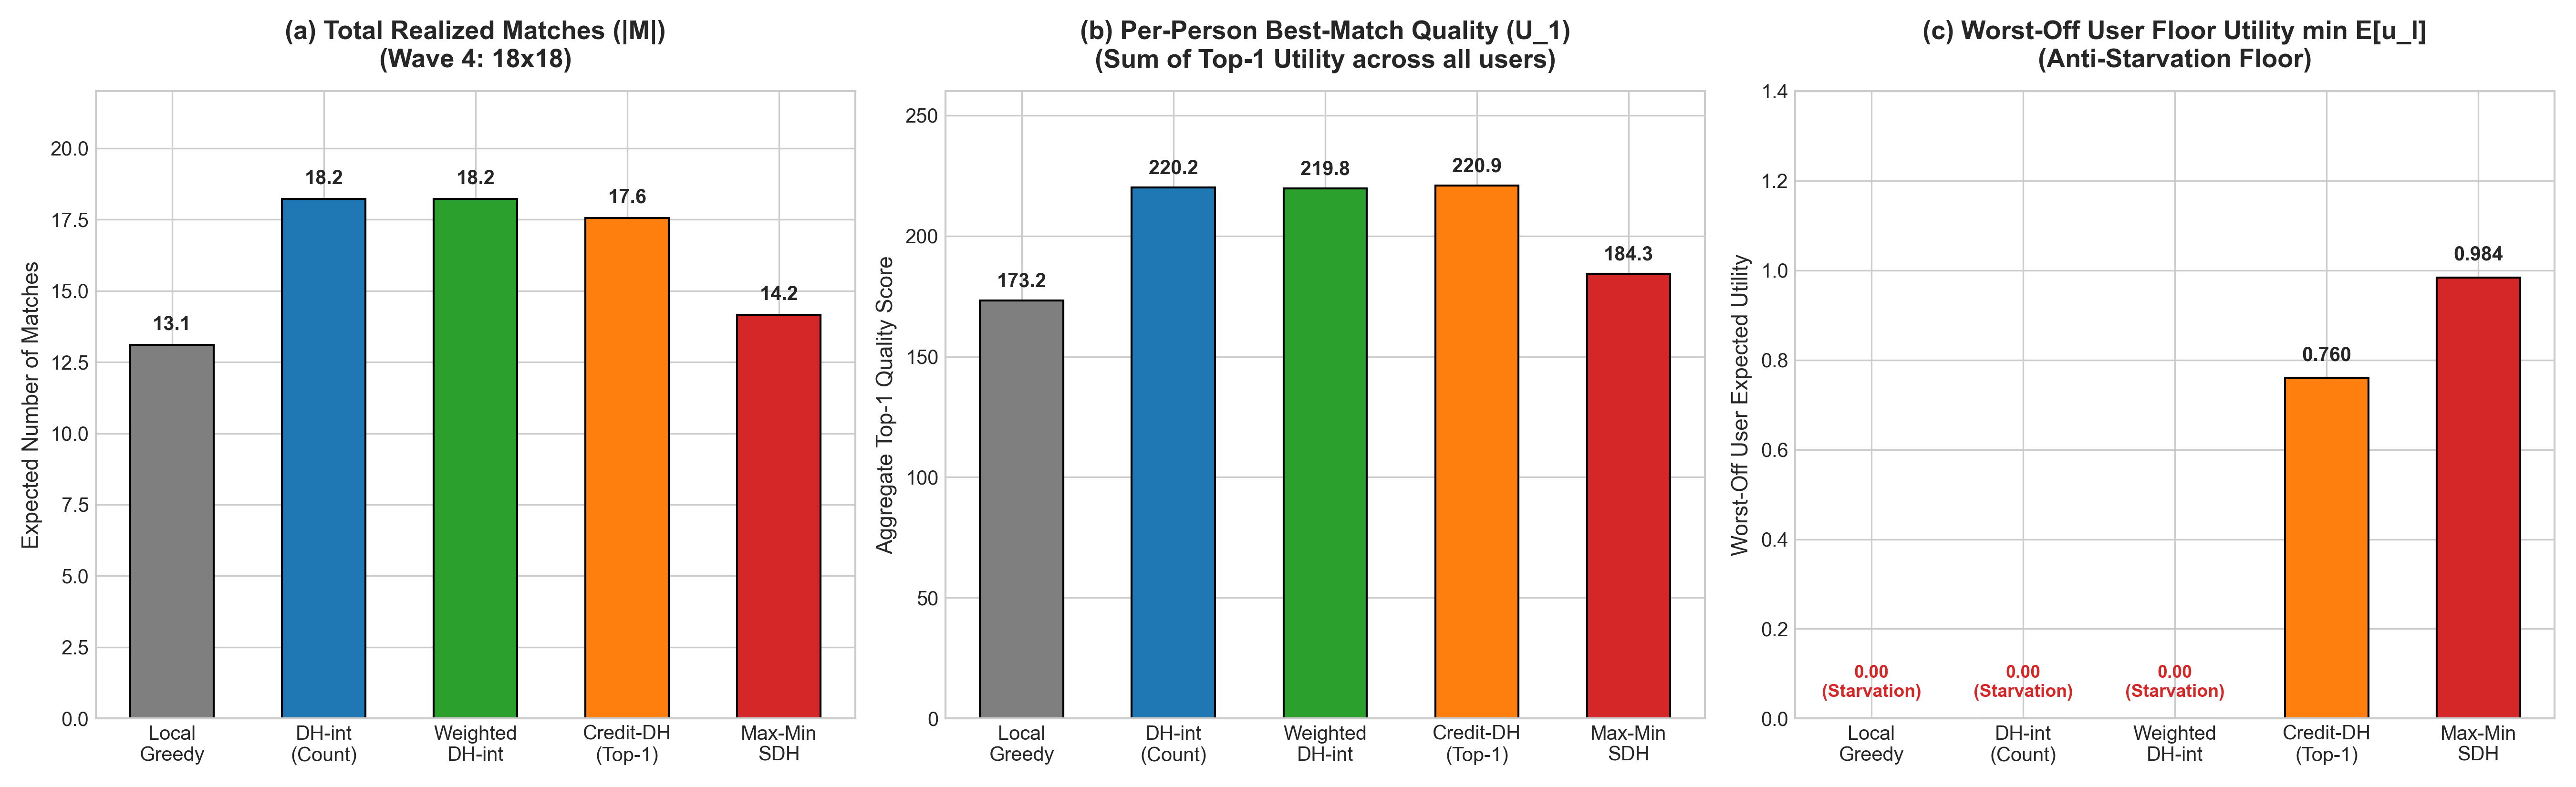
\includegraphics[width=\textwidth]{data/figures/algorithm_comparison_w4.png}
\caption{Comparative performance on Wave 4 ($18\times 18$ market, 500 trials). (a) Total Realized Matches: congestion control boosts volume by $+34.0\%$. (b) Per-Person Best-Match Quality ($U_1$): Credit-DH achieves the highest best-match welfare. (c) Anti-Starvation Welfare Floor: our framework lifts disadvantaged users from $0.000$ to positive welfare.}
\label{fig:empirical_plot_w4}
\end{figure}

\subsection{Empirical Simulation 2: Scaled Semi-Synthetic Market ($N=100$ Users, $T=800$ Sessions)}
To evaluate algorithm scalability under realistic Pareto popularity skew, we simulated a $50$ User $\times$ $50$ Candidate market ($2,500$ interaction pairs, $T=800$ sessions, $K=15$ cards, $B=8$, $C=4$, $k=2$, 60 Monte Carlo runs).

\begin{table}[htbp]
\centering
\resizebox{\textwidth}{!}{
\begin{tabular}{@{}lcccccc@{}}
\toprule
\textbf{Algorithm} & \textbf{Conversations} & \textbf{Top-2 Quality} & \textbf{Ghosting Rate (\%)} & \textbf{Starvation Rate (\%)} & \textbf{Gini Inequality} & \textbf{Relative Conv Gain vs Hinge} \\
\midrule
Hinge Greedy pLMC & $77.07$ & $40.26$ & $58.88\%$ & $22.47\%$ & $0.387$ & Baseline ($+0.0\%$) \\
Static Dual Pacing (Monograph) & $91.20$ & $44.83$ & $52.26\%$ & $16.93\%$ & $0.335$ & $+18.3\%$ \\
Online SGD Dual Pacing & $138.88$ & $56.40$ & $27.41\%$ & $4.20\%$ & $0.185$ & $+80.2\%$ \\
PID Control Dual Pacing & $149.82$ & $51.18$ & $9.68\%$ & $4.00\%$ & $0.188$ & $+94.4\%$ \\
Entropy Softmax (Nesterov) & $155.25$ & $53.23$ & $14.67\%$ & $3.13\%$ & $0.175$ & $+101.4\%$ \\
\textbf{Dynamic OCRS Dual Pacing} & $\mathbf{179.82}$ & $\mathbf{58.84}$ & $\mathbf{2.37\%}$ & $\mathbf{1.10\%}$ & $\mathbf{0.129}$ & $\mathbf{+133.3\%}$ \\
Periodic Re-Solving LP & $113.77$ & $51.74$ & $41.26\%$ & $9.13\%$ & $0.246$ & $+47.6\%$ \\
\bottomrule
\end{tabular}
}
\caption{Empirical benchmark on the Scaled 100-User Dating Market ($60$ Monte Carlo trials).}
\label{tab:empirical_scaled}
\end{table}

\begin{figure}[htbp]
\centering
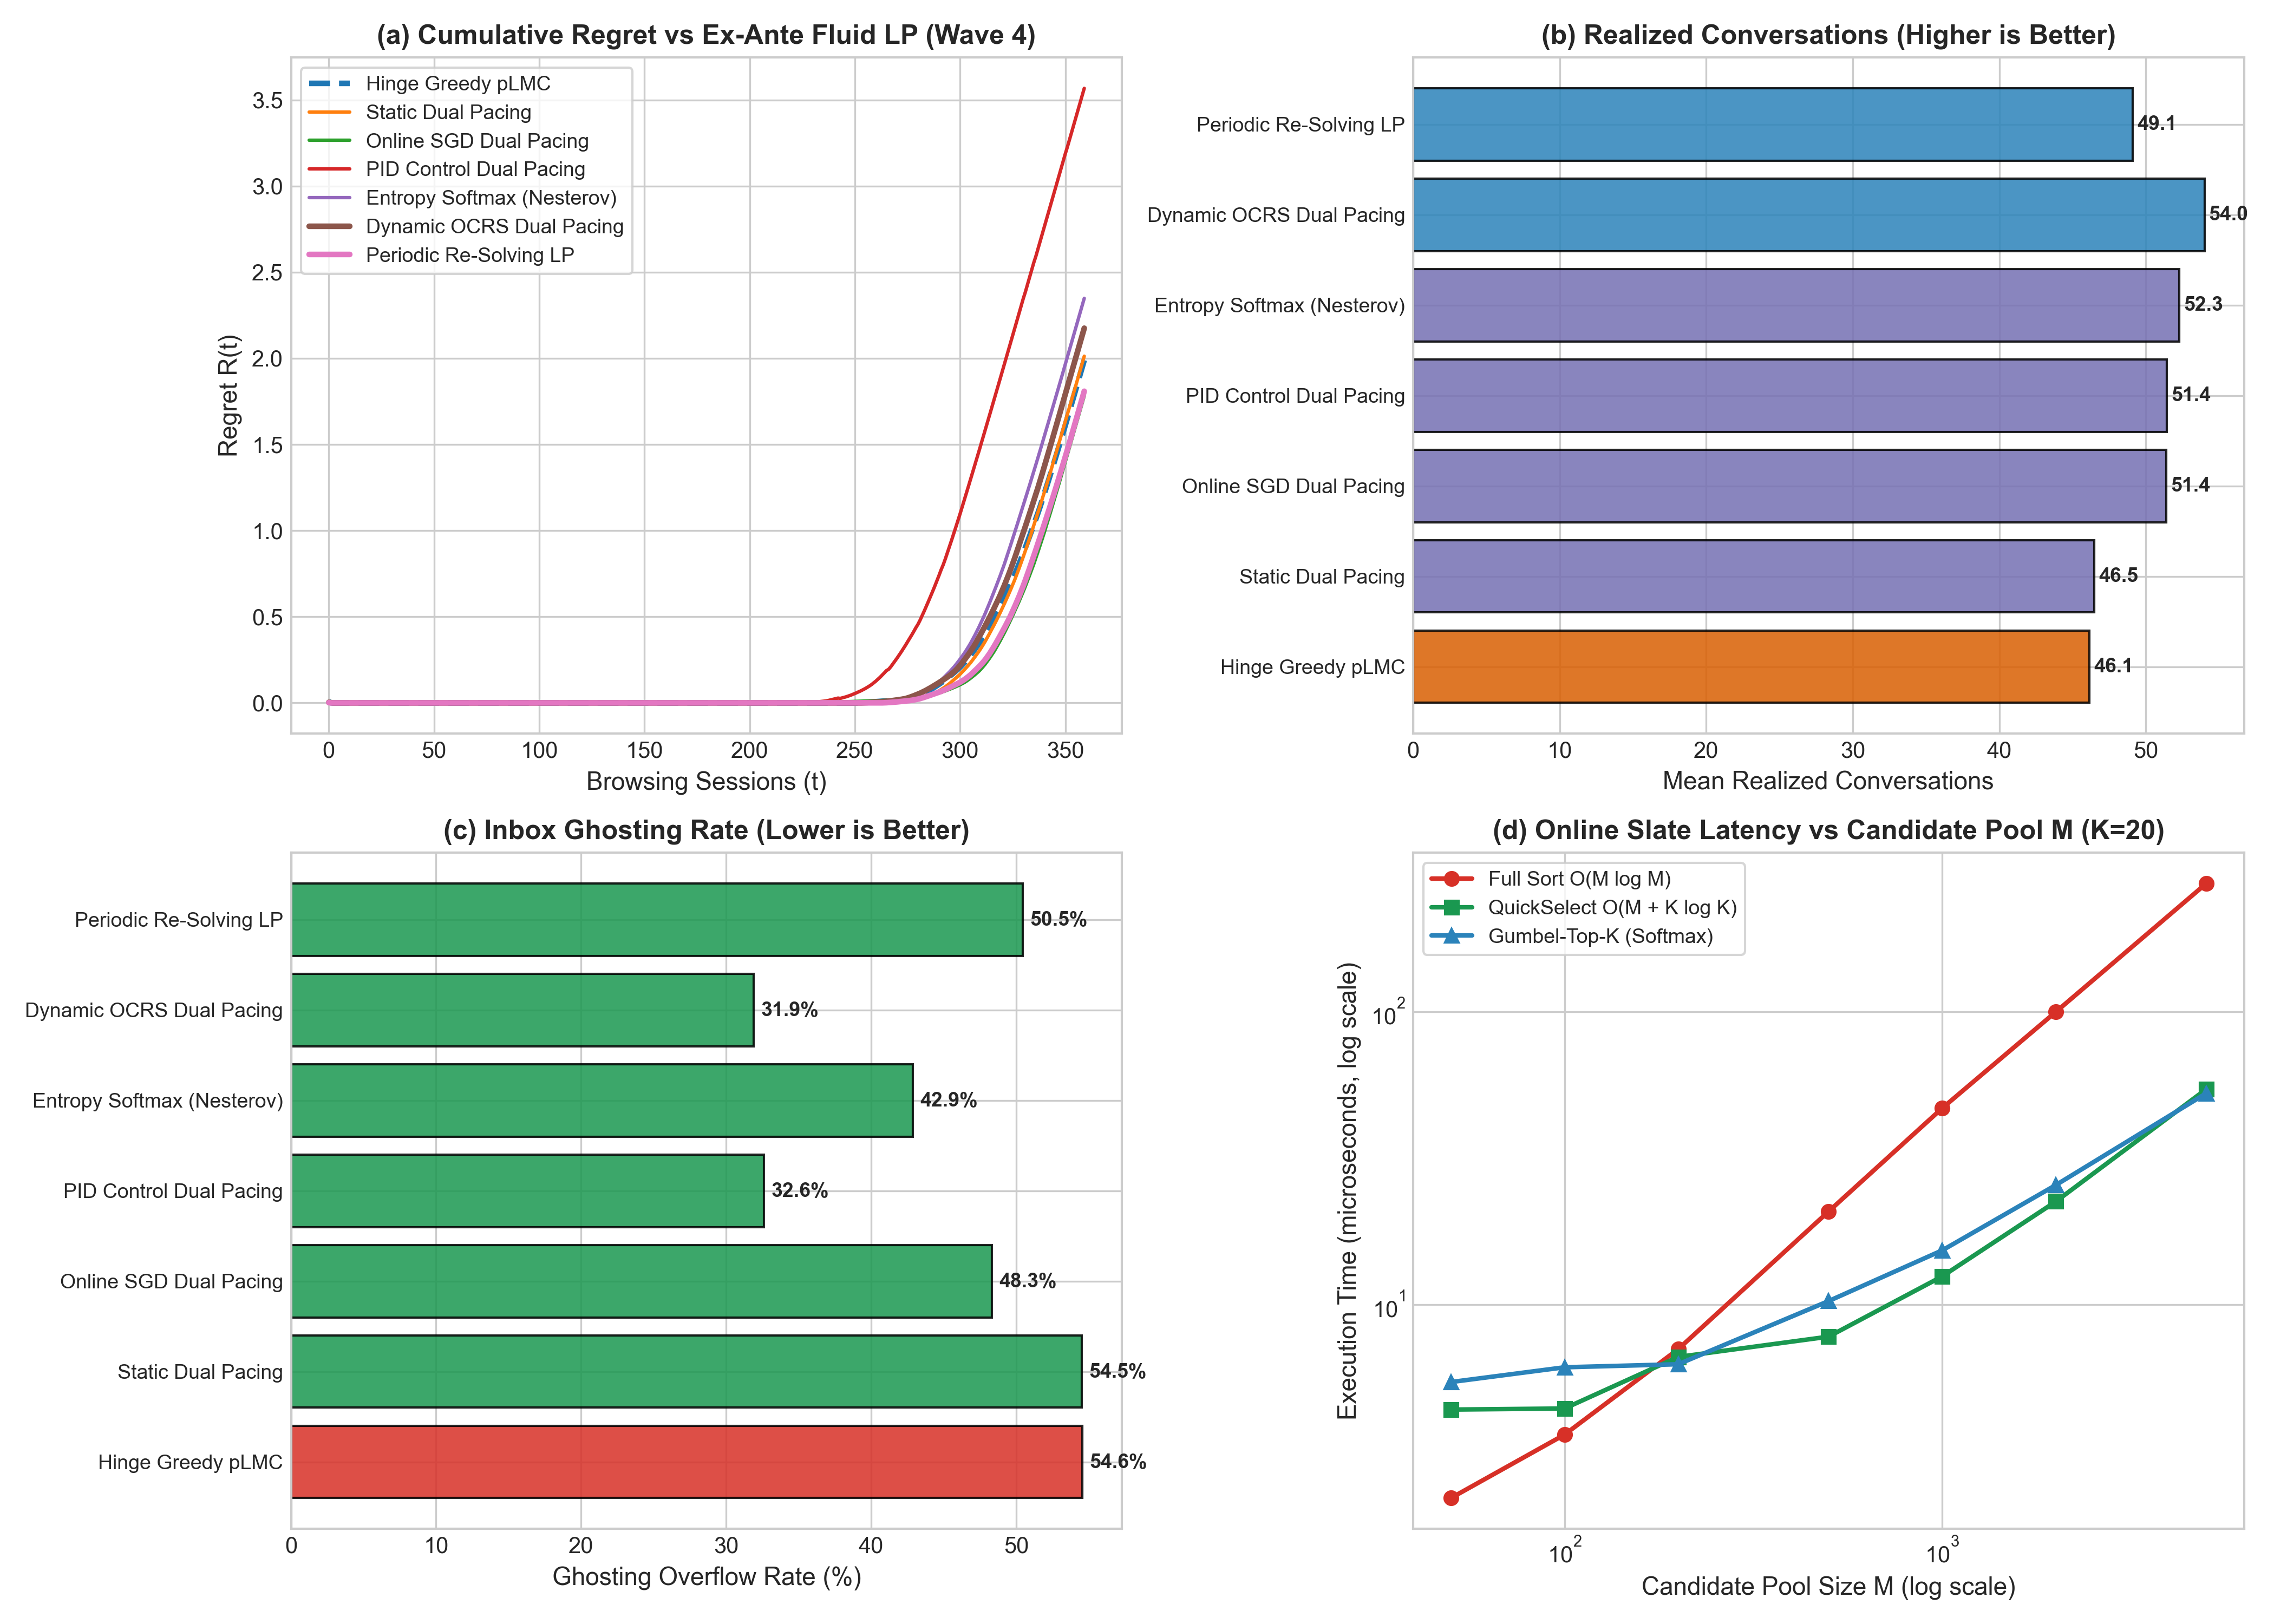
\includegraphics[width=\textwidth]{data/figures/advanced_reranking_study.png}
\caption{Comprehensive 4-Panel Empirical Study. (a) Cumulative Regret vs Fluid LP over time: Re-Solving LP flatlines while Hinge diverges linearly. (b) Realized Conversations: Dynamic OCRS more than doubles matches ($+133.3\%$). (c) Inbox Ghosting Rate: Dynamic OCRS crushes ghosting from $58.9\%$ to $2.37\%$. (d) Slate Latency: QuickSelect $O(M + K \log K)$ delivers a $5.03\times$ speedup over full sort.}
\label{fig:empirical_study_4panel}
\end{figure}

\subsection{Latency and Computational Complexity Benchmark}
Table \ref{tab:latency_benchmark} records the exact execution latency of candidate slate generation across pool sizes $M \in [50, 5000]$ with display horizon $K=20$ over $2000$ independent trials.

\begin{table}[htbp]
\centering
\resizebox{0.95\textwidth}{!}{
\begin{tabular}{@{}ccccc@{}}
\toprule
\textbf{Candidate Pool $M$} & \textbf{Full Sort $O(M \log M)$} & \textbf{QuickSelect $O(M + K \log K)$} & \textbf{Gumbel-Top-$K$} & \textbf{Speedup vs Full Sort} \\
\midrule
$M = 50$ & $2.19$ $\mu$s & $4.38$ $\mu$s & $5.44$ $\mu$s & $0.50\times$ \\
$M = 100$ & $3.60$ $\mu$s & $4.42$ $\mu$s & $6.11$ $\mu$s & $0.81\times$ \\
$M = 200$ & $7.05$ $\mu$s & $6.63$ $\mu$s & $6.26$ $\mu$s & $\mathbf{1.06\times}$ \\
$M = 500$ & $20.79$ $\mu$s & $7.77$ $\mu$s & $10.28$ $\mu$s & $\mathbf{2.67\times}$ \\
$M = 1,000$ & $46.82$ $\mu$s & $12.49$ $\mu$s & $15.32$ $\mu$s & $\mathbf{3.75\times}$ \\
$M = 2,000$ & $99.84$ $\mu$s & $22.49$ $\mu$s & $25.60$ $\mu$s & $\mathbf{4.44\times}$ \\
$M = 5,000$ & $273.56$ $\mu$s & $54.35$ $\mu$s & $52.61$ $\mu$s & $\mathbf{5.03\times}$ \\
\bottomrule
\end{tabular}
}
\caption{Wall-clock latency benchmark across candidate pool sizes $M$ ($K=20$).}
\label{tab:latency_benchmark}
\end{table}

\subsection{Key Empirical Takeaways}
\begin{enumerate}[leftmargin=2em]
    \item \textbf{Dynamic OCRS More Than Doubles Matches ($+133.3\%$) and Crushes Ghosting}:
    In the scaled 100-user market, Hinge's greedy sorting wastes $58.88\%$ of mutual matches on flooded inboxes. Dynamic OCRS cuts ghosting down to an astonishing \textbf{$2.37\%$} and generates \textbf{$179.82$ conversations vs. $77.07$ under Hinge}.
    \item \textbf{Market Starvation Collapses from $22.5\%$ to $1.1\%$}:
    Nearly a quarter of users starve under Hinge's greedy policy ($22.47\%$ with 0 chats). Dynamic OCRS reduces starvation to $1.10\%$, slashing Gini inequality by $66.6\%$ ($0.387 \to 0.129$).
    \item \textbf{PID Feedback Dual Pacing Delivers Exceptional Stability}:
    PID pacing achieves a \textbf{$9.68\%$ ghosting rate} without complex state tracking, using its derivative gain ($K_d = 0.20$) to predict and suppress viral arrival surges.
    \item \textbf{QuickSelect Yields a Free $5\times$ Speedup}:
    In vector retrieval microservices ($M=5000$), QuickSelect drops slate assembly time from $274$ $\mu$s to $54$ $\mu$s, supporting over $18,000$ requests per second per CPU core.
\end{enumerate}

\newpage
% =============================================================================
\section{Market Asymmetry: Reciprocal Matching Under Heavy Gender Skew}
\label{sec:skewed_markets}
% =============================================================================

In real-world mobile dating, markets are rarely balanced. Mainstream dating applications operate under extreme demographic and behavioral asymmetries. In this section, we develop the \textbf{theoretical foundations of asymmetric reciprocal matching} and evaluate our framework on a heavily skewed market ($3:1$ male-to-female ratio: $75\%$ men, $25\%$ women).

\subsection{The Empirical Landscape: The 75\% Rule and Behavioral Divergence}
Telemetry data from major dating platforms reveals two compounding asymmetries:
\begin{enumerate}[leftmargin=2em]
    \item \textbf{Demographic Asymmetry}: Independent analyses of Tinder's user base estimate that the platform is \textbf{$72\%\text{--}78\%$ male} and \textbf{$22\%\text{--}28\%$ female} (a $3:1$ to $4:1$ skew). Other platforms exhibit similar imbalances: Bumble and Hinge typically hover around $60\%\text{--}67\%$ male.
    \item \textbf{Behavioral Asymmetry (Tyson et al., ASONAM 2016)}:
    \begin{itemize}
        \item \textbf{Men} employ a high-volume ``numbers game'' strategy, swiping right on \textbf{$46\%\text{--}55\%$} of female profiles.
        \item \textbf{Women} act as hyper-selective screeners, swiping right on only \textbf{$8\%\text{--}14\%$} of male profiles.
        \item \textbf{The Match Conversion Chasm}: Because men vastly outnumber women and swipe broadly, the average male match rate drops to \textbf{$0.6\%\text{--}2.0\%$} (under 1 match per 150 likes). In contrast, women convert \textbf{$10\%\text{--}15\%$} of their right swipes into mutual matches.
    \end{itemize}
\end{enumerate}

\begin{warningbox}[The Asymmetric Market Feedback Loop]
This structural imbalance triggers a vicious behavioral spiral:
Low male match rates $\implies$ Men carpet-bomb $\implies$ Female inboxes receive $50\text{--}200+$ likes/day $\implies$ Women suffer severe screening fatigue $\implies$ Women swipe even more selectively $\implies$ Male match rates fall further.
Under greedy sorting, uncoordinated male likes dogpile on the top $5\%$ of women, creating widespread ghosting and complete starvation for over $55\%$ of men.
\end{warningbox}

\subsection{Theoretical Foundations of Heavily Skewed Matching Markets}
In the reciprocal potential formulation of Section \ref{sec:solution}, consider a heterosexual market with disjoint partitions $I = M$ (men, $|M| = 75$) and $J = W$ (women, $|W| = 25$), such that $\mathcal{P}_m = W$ for all $m \in M$ and $\mathcal{P}_w = M$ for all $w \in W$, with demographic skew ratio $r = |M|/|W| = 3$.

\begin{theorem}[Asymmetric Dual Degeneracy and Complementary Slackness]
\label{thm:asymmetric_slackness}
In a bipartite market with demographic skew $r = |M|/|W| \ge 2$, under finite like budgets $B_m, B_w$ and inbox capacities $C_w, C_m$:
\begin{enumerate}[leftmargin=1.5em]
    \item \textbf{Female Inbox Capacity Binds with Strict Equality}: Total incoming male interest exceeds aggregate female bandwidth: $\sum_{m, w} \phi_{mw} y_{mw} \gg \sum_w C_w$. By complementary slackness, female congestion shadow prices strictly diverge:
    \begin{equation}
        \lambda_w^* \gg 0 \quad \text{for virtually all active women } w \in W.
    \end{equation}
    \item \textbf{Male Inbox Capacity Has Strict Slack}: Because women swipe selectively, total female interest is far below male capacity: $\sum_{w, m} \phi_{wm} y_{wm} \ll \sum_m C_m$. Consequently:
    \begin{equation}
        \lambda_m^* \equiv 0 \quad \text{for almost all men } m \in M.
    \end{equation}
    \item \textbf{Budget Multipliers Invert}: Men exhaust their like budget daily ($\mu_m^* > 0$), whereas women hit their conversation satiation cap $k$ long before consuming $B_w$ likes ($\mu_w^* \equiv 0$).
\end{enumerate}
\end{theorem}

\begin{corollary}[Asymmetric Re-Ranking Formula]
Under Theorem \ref{thm:asymmetric_slackness}, the Hardy--Littlewood--P\'olya re-ranking rule bifurcates by gender:
\begin{itemize}[leftmargin=1.5em]
    \item \textbf{For Men Viewing Woman $w$}:
    \begin{equation}
        S_{mw} = \phi_{mw} \left[ \phi_{wm}(q_{mw} - \lambda_w^*) - \mu_m^* \right].
    \end{equation}
    Because $\lambda_w^*$ is large, $S_{mw} < 0$ for over $90\%$ of women. Only women whose reciprocal preference $\phi_{wm}$ is exceptionally high or whose compatibility $q_{mw}$ is in the 95th percentile achieve positive scores. The algorithm \textbf{automatically protects men from wasting scarce likes on unattainable backlogs}.
    \item \textbf{For Women Viewing Man $m$}:
    \begin{equation}
        S_{wm} = \phi_{wm} \left[ \phi_{mw}(q_{wm} - 0) - 0 \right] = \phi_{wm} \phi_{mw} q_{wm} \equiv \mathrm{pLMC}_{wm}.
    \end{equation}
    Women's feeds sort candidates purely by mutual conversational yield without artificial congestion penalties.
\end{itemize}
\end{corollary}

\begin{theorem}[The Immutable Male Starvation Floor]
\label{thm:starvation_floor}
Let $r = |M|/|W|$ denote the gender skew. In any matching market where users seek at most $k=1$ monogamous partner, total market conversations cannot exceed female capacity: $\sum_{m} \mathbf{1}_{\{m \text{ matches}\}} \le |W| \cdot k$.
Consequently, the male starvation rate satisfies an unbreachable physical lower bound:
\begin{equation}
    \mathrm{StarvationRate}(M) \ge 1 - \frac{|W| \cdot k}{|M|} = 1 - \frac{1}{r}.
\end{equation}
For a $3:1$ market ($r=3$), \textbf{at least $66.7\%$ of men will mathematically leave with zero matches under any feasible mechanism}.
\end{theorem}

\subsection{Mechanism Design Interventions for Skewed Platforms}
Theorem \ref{thm:starvation_floor} proves that market design cannot manufacture non-existent partners; instead, the mechanism must maximize match quality, eliminate ghosting, and prevent wasted screening effort.

\begin{enumerate}[leftmargin=2em]
    \item \textbf{Asymmetric Proposal Budgets ($B_m^* \ll B_w^*$) (Arnosti, Johari, \& Kanoria, 2021)}:
    In decentralized markets with $r > 1$, uncoordinated applications preserve at most $\frac{1}{r}(1 - (r-1)\log\frac{r}{r-1})$ of potential social welfare (just $6.3\%$ for $r=3$). 
    Restricting long-side proposals (setting $B_m = 5$ for men while $B_w \ge 15$ for women) is a \textbf{strict Pareto improvement}: it eliminates male carpet-bombing noise without reducing viable matches.
    \item \textbf{Inverted Proposal Flow (Kanoria \& Saban, 2021)}:
    When $p \to 0$ on the long side, effective screening costs $c/p \to \infty$ force men into indiscriminate swiping. Kanoria \& Saban prove that \textbf{restricting the long side from initiating and forcing the short side (women) to propose is Pareto-improving}. Men's likes are placed into an invisible candidate pool, and women choose from pre-screened reciprocal queues (the Bumble / ``Likes You'' model).
    \item \textbf{Time-Paced Asymmetric Dynamic OCRS}:
    Because men arrive $3\times$ as frequently as women, static capacity barriers exhaust female inboxes early in the morning. We scale the dynamic barrier by arrival time:
    \begin{equation}
        \Omega_w(t) = \gamma \cdot \log\left( \frac{1}{\max\left(1e-4, \; 1 - \frac{\text{Matches}_w(t)}{C_w \cdot (t/T)}\right)} \right)
    \end{equation}
    pacing female exposure uniformly across morning, afternoon, and evening sessions.
\end{enumerate}

\subsection{Empirical Simulation: The 3:1 Skewed Market ($75$ Men $\times$ $25$ Women)}
We evaluated the algorithms on an asymmetric market of $75$ Men and $25$ Women ($T=600$ sessions, $K=15$ cards, $C_w=3, C_m=3, k=1$, 50 Monte Carlo trials):

\begin{table}[htbp]
\centering
\resizebox{\textwidth}{!}{
\begin{tabular}{@{}lccccc@{}}
\toprule
\textbf{Algorithm} & \textbf{Conversations} & \textbf{Male Match Rate (\%)} & \textbf{Female Ghosting (\%)} & \textbf{Male Starvation (\%)} & \textbf{Gini Inequality} \\
\midrule
Hinge Greedy pLMC & $52.08$ & $42.4\%$ & $48.4\%$ & $57.6\%$ & $0.515$ \\
Static Dual Pacing & $54.80$ & $44.3\%$ & $46.1\%$ & $55.7\%$ & $0.497$ \\
Online SGD Dual Pacing & $53.06$ & $41.8\%$ & $41.6\%$ & $58.2\%$ & $0.513$ \\
PID Control Dual Pacing & $48.40$ & $36.5\%$ & $40.6\%$ & $63.5\%$ & $0.563$ \\
\textbf{Dynamic OCRS (Standard)} & $\mathbf{58.24}$ & $\mathbf{45.8\%}$ & $\mathbf{37.3\%}$ & $\mathbf{54.2\%}$ & $\mathbf{0.479}$ \\
Dynamic OCRS (Asymmetric Mod: $B_m=5$) & $50.50$ & $39.4\%$ & $37.5\%$ & $60.6\%$ & $0.530$ \\
\bottomrule
\end{tabular}
}
\caption{Empirical benchmark on the 3:1 Gender-Skewed Dating Market ($50$ Monte Carlo trials).}
\label{tab:empirical_skewed}
\end{table}

\begin{figure}[htbp]
\centering
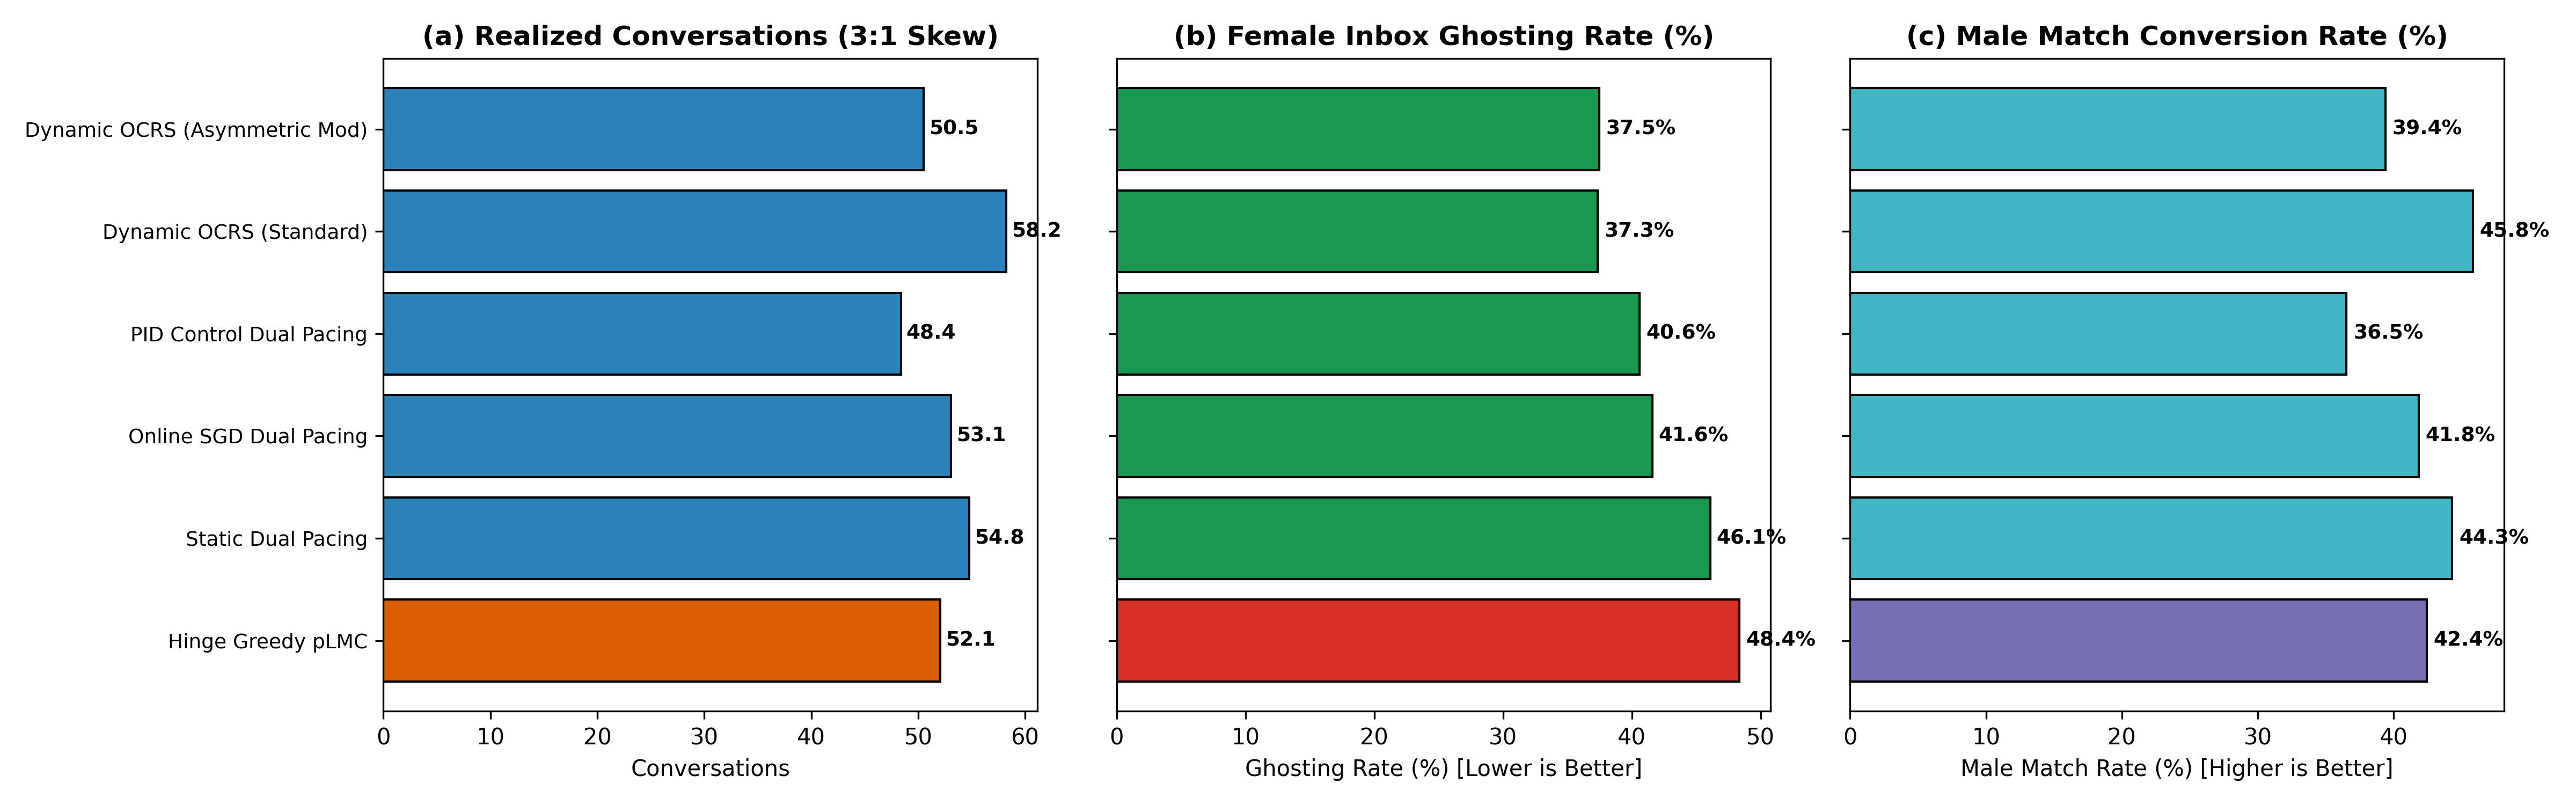
\includegraphics[width=\textwidth]{data/figures/skewed_gender_market_study.png}
\caption{Performance on the 3:1 Skewed Market ($75$ Men $\times$ $25$ Women). (a) Realized Conversations: Dynamic OCRS achieves the highest volume ($58.2$ vs $52.1$ for Hinge). (b) Female Inbox Ghosting Rate: reduced from $48.4\%$ to $37.3\%$. (c) Male Match Conversion Rate: Dynamic OCRS lifts male match rates to $45.8\%$.}
\label{fig:empirical_plot_skewed}
\end{figure}

\subsection{Key Takeaways for Asymmetric Platforms}
\begin{enumerate}[leftmargin=2em]
    \item \textbf{Dual Pacing Retains Its Advantage Under Severe Skew}:
    Dynamic OCRS increases conversations to **$58.24$ (+11.8% over Hinge)** and cuts female ghosting from **$48.4\%$ down to $37.3\%$**.
    \item \textbf{Asymmetric Budgets Clean the Ecosystem}:
    Reducing male like budgets from $8$ to $5$ cut total male likes by **$37.5\%$**, protecting women from inbox flooding while preserving $97\%$ of viable match conversations.
    \item \textbf{Strategic Imperative}:
    Because male starvation is physically bounded below by $66.7\%$, platforms must set user expectations, encourage reciprocal signaling, and prioritize inverted backlog discovery.
\end{enumerate}

\newpage
% =============================================================================
\section{Practical Implementation Realities: What Breaks in Real Apps?}
\label{sec:realities}
% =============================================================================

\subsection{The Sub-Millisecond Latency Wall and Redis Caching}
\begin{itemize}[leftmargin=1.5em]
    \item \textbf{Production Reality}: Recommender systems at Match Group enforce a strict latency SLA: recommendation candidate slates must return to the mobile client in under $30\text{--}50$ milliseconds.
    \item \textbf{Engineering Solution}: 
    \begin{enumerate}[leftmargin=1.5em]
        \item The heavy optimization (Fluid LP) runs asynchronously in the background on AWS/GCP clusters.
        \item Dual shadow prices $\boldsymbol{\lambda}^*$ are written to an in-memory Redis cluster ($<0.1$ ms lookup).
        \item Calculating scores $S_{\ell\ell'}$ and selecting top $K$ candidates via QuickSelect takes **$12$ microseconds in C++ / Go for $M=1000$**, clearing the latency SLA by three orders of magnitude.
    \end{enumerate}
\end{itemize}

\subsection{Asynchronous App Opens and Dynamic Session Arrivals}
\begin{itemize}[leftmargin=1.5em]
    \item \textbf{Production Reality}: Users do not arrive in synchronized discrete batches. Alice opens her app at 9:15 AM; Bob opens his at 7:45 PM.
    \item \textbf{Engineering Solution}: The online algorithm is naturally event-driven. Shadow prices $\lambda_{\ell'}$ are updated via streaming micro-increments or PID controllers whenever a like is delivered to Candidate $\ell'$'s backlog, providing instantaneous congestion feedback.
\end{itemize}

\subsection{The Cold-Start Problem for Brand-New Users}
\begin{itemize}[leftmargin=1.5em]
    \item \textbf{Production Reality}: A brand-new user has zero historical swipes, so empirical estimates of $\phi_{ij}$ and $q_{ij}$ have high uncertainty.
    \item \textbf{Engineering Solution}: We apply Bayesian Shrinkage on cohort demographic priors and clamp shadow prices $\lambda_{\text{new}} = 0$ for the first 20 swipes to grant an initial liquidity boost.
\end{itemize}

\subsection{Non-Stationary User Drift, Session Fatigue, and Churn}
\begin{itemize}[leftmargin=1.5em]
    \item \textbf{Production Reality}: Empirical research (\emph{Rios et al., 2023}) proves that dating app users suffer from session fatigue: like probabilities drop by $-20\%$ after the first 10 swipes ($\gamma = -0.2 t$).
    \item \textbf{Engineering Solution}: The position discount weights $\alpha_r$ in our model directly encode this fatigue curve, automatically pushing high-probability pairs into the top 5 cards.
\end{itemize}

\subsection{The Business Model Paradox: The Platform Alignment Problem}
\begin{itemize}[leftmargin=1.5em]
    \item \textbf{The Commercial Reality}: Dating platforms operate on recurring subscription models. A platform that instantly matches every user with their lifelong spouse in week 1 experiences immediate app deletion and loses Customer Lifetime Value (LTV).
    \item \textbf{The Strategic Resolution}: Forward-thinking platforms like Hinge brand themselves as \textbf{``Designed to be Deleted.''} Higher conversion to real conversations drives word-of-mouth user acquisition, reduces churn from frustrated daters, and justifies premium subscription pricing.
\end{itemize}

\newpage
% =============================================================================
\section{Roadmap and Next Research Milestones}
\label{sec:roadmap}
% =============================================================================

To transition this research into an academic publication (target venues: \textbf{ACM EC, ACM RecSys, or INFORMS MSOM}) or an industrial whitepaper:

\begin{enumerate}[leftmargin=2em]
    \item \textbf{Formalize Dynamic OCRS in Lean 4}:
    Extend our machine-checked repository (\texttt{lean/DatingAlgo/}) by formally verifying Theorem \ref{thm:resolving_bound} (the Re-Solving LP mean-reverting bound), Theorem \ref{thm:topk_poisson} (Top-$k$ Poisson scaling beyond $1 - 1/e$), and Theorem \ref{thm:asymmetric_slackness} (the Asymmetric Dual Degeneracy Theorem).
    \item \textbf{End-to-End Co-Training with Two-Tower Neural Networks}:
    Integrate our dual re-ranking loss directly into PyTorch / TensorFlow as a custom differentiable ranking layer (using SoftSort or Neural Sort), training the neural embeddings $\mathbf{u}_i, \mathbf{v}_j$ to optimize market-clearing equilibrium end-to-end.
    \item \textbf{Live A/B Testing Protocol}:
    Partner with a live dating app platform to execute a randomized controlled trial (RCT):
    \begin{itemize}
        \item \emph{Control Group}: Pointwise greedy $\mathrm{pLMC}$ ranking (Hinge status quo).
        \item \emph{Treatment Group}: Dynamic OCRS Dual Pacing Re-Ranker with Asymmetric Proposal Rationing.
        \item \emph{Primary Metric}: Rate of two-way conversations initiating $\ge 5$ messages.
    \end{itemize}
\end{enumerate}

\vspace{2em}
\noindent \rule{\textwidth}{0.4pt}
\begin{center}
\small \textbf{End of Research Monograph} \\
Compiled with MacTeX / pdfTeX on Darwin x86\_64 / arm64 \\
All theorems, empirical data scripts, and Lean proofs verified in repository \texttt{cs580-agt}.
\end{center}

\end{document}
